\section{Actual Task Allocation(ps)}
In the real work environment, the unexpected situation happens at all time. 
Each members of the group faced different problems.
Some problem was easy to solved but some was very difficult and time consuming. 
The back up plan and unplanned problem solving skills is needed. 
Although many problems happened, but all the team members have been flexible to support each other and most main problems have been solved. Figure\ref{final task allocation} shows an actual work that each member has done in the project

\begin{figure}[H]
        \centering
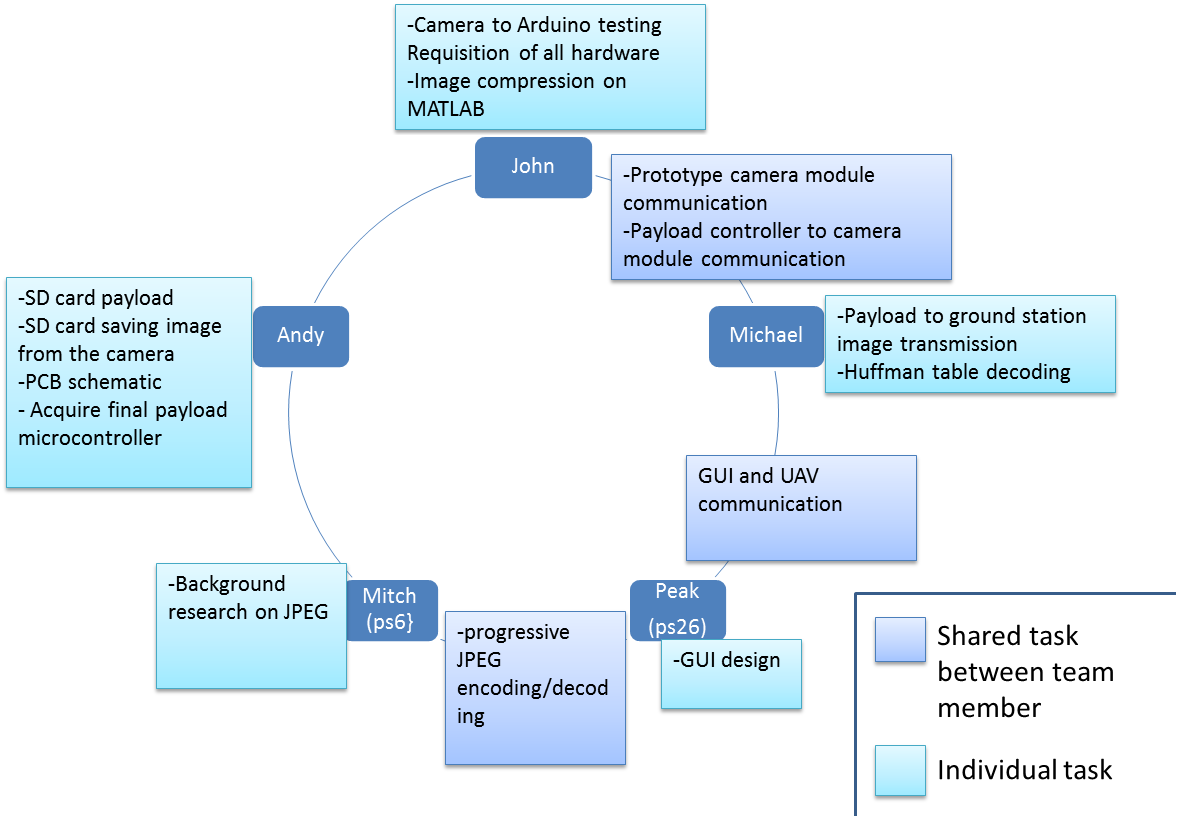
\includegraphics[width=1.0\textwidth]{figures/finalWorkAllocation.png} 
        \captionof{figure}{A diagram show a final work allocation of the team}
        \label{final task allocation}
\end{figure}

Figure\ref{systemBlocD} shows a block diagram of the whole system that the developers has slitted in to blocks of tasks. 

The camera module and other hardware have uncontrollable acquiring time. 
Some of the group members has problem with the delay of the hardware deliveries. Therefore, the time has to extended longer than the gantt chart. 
The solution to this is the software has been developed according to the camera sheet of the hardware. 
And at this stage, the background reading is very necessary so the developers has used this waiting time to plan and develop the software, so when the components arrive, all the task can be implemented.

The task that depend on acquiring the camera are the communication between the payload and the camera,prototype camera module, and image encoding. 
The problem that the developers have is the camera delivered is a faulty.
These tasks has been suspended until the camera have arrived.  
Therefore, the new camera has to be purchased and the allocation of work is necessary. 
There are part that is not depended on the hardware such as encoding/decoding images, and ground station software. 
So the members who were assigning to work on the camera has been allocate to do the software part first.

The payload controller has the problem with the hardware part of the UAV. 
It did not respond to the UAV signal at first. 
Therefore, we assign another group member to support this problems. 
The task leader of this has been assigned to do another software module which have to be implemented. 
This problem also need a support from the customer to update the UAV firmware. 
After problem have been noticed, it has been solved successfully. 

The SD card memory task was considered as a small task in the planned work, but in the real implementation it is very important. 
Therefore, we assign on of the member responsible to this task. 
The SD started to implemented after the camera have been arrive and implemented correctly. 

Because there is only one camera purchased, only one member of the team assign to keep the camera. 
There are problems with the cameras including the delay of deliveries, and camera faulty. 
The task leader of this has been assign to research on the progressive image on MATLAB in order to make a prototype presentation of a compression image taken. 
The task has been delayed from the time set to an individual. 
But after the second working camera arrived, the task has been done beautifully and there is enough time to combine with other tasks.